\chapter{Marco teórico}
\label{ch:marco_teorico}

\paragraph*{}En este capítulo se presentan los conceptos teóricos sobre los que se apoya el proyecto. Al tratarse de una ampliación de un dashboard ya existente, no se parte desde cero, sino desde una base previa centrada en el análisis de supervivencia aplicado al abandono académico universitario. Por ello, el marco teórico se organiza comenzando por los fundamentos generales de esta técnica, continúa con los modelos clásicos ya presentes en el sistema original y, finalmente, introduce las técnicas incorporadas en esta nueva versión.

\section{Fundamentos del análisis de supervivencia}
\paragraph*{}El análisis de supervivencia es un conjunto de técnicas estadísticas orientadas al estudio del tiempo que transcurre hasta que ocurre un determinado evento. Aunque el término ``supervivencia'' procede principalmente del ámbito médico, donde se utiliza para analizar el tiempo hasta el fallecimiento, la recuperación o la recaída de un paciente, su aplicación no se limita a ese contexto. También se emplea en ingeniería para estudiar la vida útil de componentes, en economía para analizar la duración de determinados procesos y, más recientemente, en educación para estudiar fenómenos como el abandono académico, es decir, contextos muy diferentes pero con algo en común: todos se preguntan cuánto tiempo tarda en ocurrir algo.

\paragraph*{}En este Trabajo Fin de Grado, ese ``algo'' es el abandono universitario. La idea principal no consiste únicamente en saber si un estudiante abandona o no, sino en analizar cuándo se produce ese abandono y qué factores pueden estar relacionados con él. Este matiz es importante, porque permite observar el fenómeno como un proceso temporal y no como un resultado aislado. Dicho de forma sencilla, no es lo mismo detectar que un estudiante abandona al inicio de sus estudios que observar que lo hace tras un periodo prolongado de permanencia.

\paragraph*{}Uno de los conceptos clave en este tipo de análisis es la función de supervivencia. Esta función representa la probabilidad de que un individuo, en este caso un estudiante, continúe en el sistema más allá de un instante determinado. Aplicado al abandono académico, permite estimar la probabilidad de permanencia del alumnado a lo largo del tiempo. A partir de esta información se pueden identificar momentos de mayor riesgo y estudiar si ciertos grupos presentan comportamientos diferentes.

\paragraph*{}Otro concepto fundamental es el de censura. En muchos estudios no se observa el evento para todos los individuos durante el periodo analizado. Por ejemplo, puede ocurrir que un estudiante siga matriculado al finalizar el periodo de observación. En ese caso, no se puede afirmar que nunca vaya a abandonar, pero sí se sabe que no lo ha hecho hasta ese momento. El análisis de supervivencia permite aprovechar este tipo de información, algo especialmente valioso en el ámbito educativo, donde las trayectorias académicas no siempre finalizan dentro del intervalo de estudio disponible.

\paragraph*{}Además, el análisis de supervivencia permite incorporar variables explicativas, también denominadas covariables, que ayudan a estudiar qué factores pueden influir en el tiempo hasta el evento. En el caso del abandono universitario, estas variables pueden estar relacionadas con aspectos académicos, personales o administrativos, como el rendimiento, la edad, el género, la discapacidad, el nivel educativo previo o los créditos cursados. Gracias a ello, el análisis no se limita a describir una curva general de permanencia, sino que puede aportar una visión más rica y útil del comportamiento de distintos perfiles de estudiantes.

\section{Técnicas clásicas de análisis de supervivencia}
\paragraph*{}El sistema desarrollado en el Trabajo Fin de Grado previo ya incorporaba varias técnicas clásicas de análisis de supervivencia. Estas técnicas constituyen la base sobre la que se apoya la ampliación actual, ya que permiten estimar la permanencia del alumnado, comparar grupos y estudiar el efecto de diferentes covariables. Aunque cada método tiene un propósito distinto, todos ellos ayudan a entender mejor el abandono académico desde una perspectiva temporal.

\subsection{Kaplan-Meier}
\paragraph*{}El estimador de Kaplan-Meier es una de las técnicas más utilizadas dentro del análisis de supervivencia. Su objetivo principal es estimar la función de supervivencia a partir de los datos observados, teniendo en cuenta tanto los casos en los que ocurre el evento como aquellos que están censurados. En el contexto de este proyecto, permite representar de forma gráfica la probabilidad de que los estudiantes permanezcan en el sistema universitario a medida que avanza el tiempo.

\paragraph*{}Una de sus ventajas es que ofrece una interpretación visual bastante directa. La curva de supervivencia permite observar en qué momentos se producen descensos más marcados, lo que puede indicar periodos de mayor riesgo de abandono. Además, puede aplicarse a distintos grupos de estudiantes, por ejemplo según género, tramo de edad o nivel educativo previo, facilitando una primera comparación entre perfiles.

\paragraph*{}No obstante, Kaplan-Meier tiene también ciertas limitaciones. Principalmente, describe la supervivencia de forma general o por grupos, pero no permite modelar de manera conjunta el efecto de varias covariables. Por ello, suele utilizarse como una herramienta inicial de exploración y visualización, complementándose con otros métodos más adecuados para analizar factores explicativos.

\subsection{Regresión de Cox}
\paragraph*{}El modelo de riesgos proporcionales de Cox permite estudiar la relación entre el tiempo hasta el evento y un conjunto de covariables. A diferencia de Kaplan-Meier, que se centra en estimar curvas de supervivencia, la regresión de Cox permite analizar cómo ciertas variables influyen en el riesgo de que ocurra el evento. En este proyecto, dicho evento se corresponde con el abandono académico.

\paragraph*{}Este modelo resulta especialmente útil porque permite interpretar el efecto de cada variable mediante razones de riesgo. De forma simplificada, una variable puede asociarse con un aumento o una disminución del riesgo de abandono. Por ejemplo, determinadas características académicas podrían estar relacionadas con una mayor probabilidad de abandonar antes, mientras que otras podrían estar asociadas con una mayor permanencia.

\paragraph*{}La regresión de Cox es una técnica muy valiosa cuando se desea estudiar el papel de varios factores al mismo tiempo. Sin embargo, parte de una hipótesis importante: los riesgos entre grupos deben ser proporcionales a lo largo del tiempo. Esto significa que el efecto relativo de las covariables se mantiene aproximadamente constante durante el periodo analizado. Si esta condición no se cumple, la interpretación del modelo puede verse afectada.

\subsection{Test de Log-Rank}
\paragraph*{}El Test de Log-Rank tiene un propósito más concreto y directo: comparar curvas de supervivencia entre grupos y determinar si las diferencias observadas son estadísticamente significativas o podrían deberse al azar. En el contexto del abandono universitario, permite preguntarse, por ejemplo, si los estudiantes de distintos tramos de edad realmente siguen trayectorias diferentes o si esa diferencia no es suficientemente relevante como para sacar conclusiones.

\paragraph*{}No explica por sí solo las causas, pero sí lanza señales. Si el test detecta diferencias significativas entre grupos, es una indicación de que esa variable merece ser estudiada con más detalle. Y ahí es donde entra en juego su papel dentro del dashboard: complementa a Kaplan-Meier, que visualiza las curvas, y a Cox, que analiza las covariables. Los tres juntos forman una base analítica coherente y bastante completa para abordar el abandono desde distintos ángulos.

\section{Técnicas incorporadas en la ampliación}
\paragraph*{}La ampliación desarrollada en este Trabajo Fin de Grado incorpora nuevas técnicas de análisis de supervivencia con el fin de enriquecer la capacidad analítica del sistema. La idea no es sustituir los métodos clásicos, sino complementarlos. Cada modelo aporta una forma distinta de mirar los datos, y esa variedad permite comparar enfoques, detectar patrones y ofrecer una interpretación más completa del fenómeno estudiado.

\subsection{Modelo exponencial}
\paragraph*{}El modelo exponencial es un modelo paramétrico de análisis de supervivencia. A diferencia de métodos como Kaplan-Meier, que no imponen una forma concreta a la función de supervivencia, los modelos paramétricos asumen una determinada distribución para describir el tiempo hasta el evento \cite{davidsonpilon2019lifelines,jackson2016flexsurv}. En el caso del modelo exponencial, se supone que el riesgo de que ocurra el evento permanece constante a lo largo del tiempo.

\paragraph*{}Esta característica lo convierte en un modelo sencillo y fácil de interpretar. Si el riesgo de abandono se considera estable durante el periodo analizado, el modelo exponencial puede ofrecer una aproximación útil. Sin embargo, esa misma simplicidad puede convertirse en una limitación cuando el riesgo cambia con el tiempo, algo que puede ocurrir en contextos educativos. Por ejemplo, puede haber periodos iniciales con mayor incertidumbre o momentos concretos del curso en los que el abandono sea más probable.

\paragraph*{}Dentro del proyecto, el modelo exponencial permite incorporar una primera aproximación paramétrica al análisis y sirve como punto de comparación frente a modelos más flexibles. Además, facilita la generación de métricas y resultados que pueden contrastarse con otras técnicas implementadas en el dashboard.

\paragraph*{}Desde el punto de vista estadístico, el modelo exponencial también puede entenderse como un caso particular del modelo de Weibull. En concreto, cuando el parámetro de forma de Weibull toma el valor \(\rho = 1\), el riesgo se mantiene constante y el modelo resultante coincide con el comportamiento exponencial. Por este motivo, el exponencial funciona bien como modelo paramétrico base: permite partir de una hipótesis sencilla y comprobar después si una formulación más flexible, como Weibull, mejora la representación del fenómeno.

\begin{figure}[H]
    \centering
    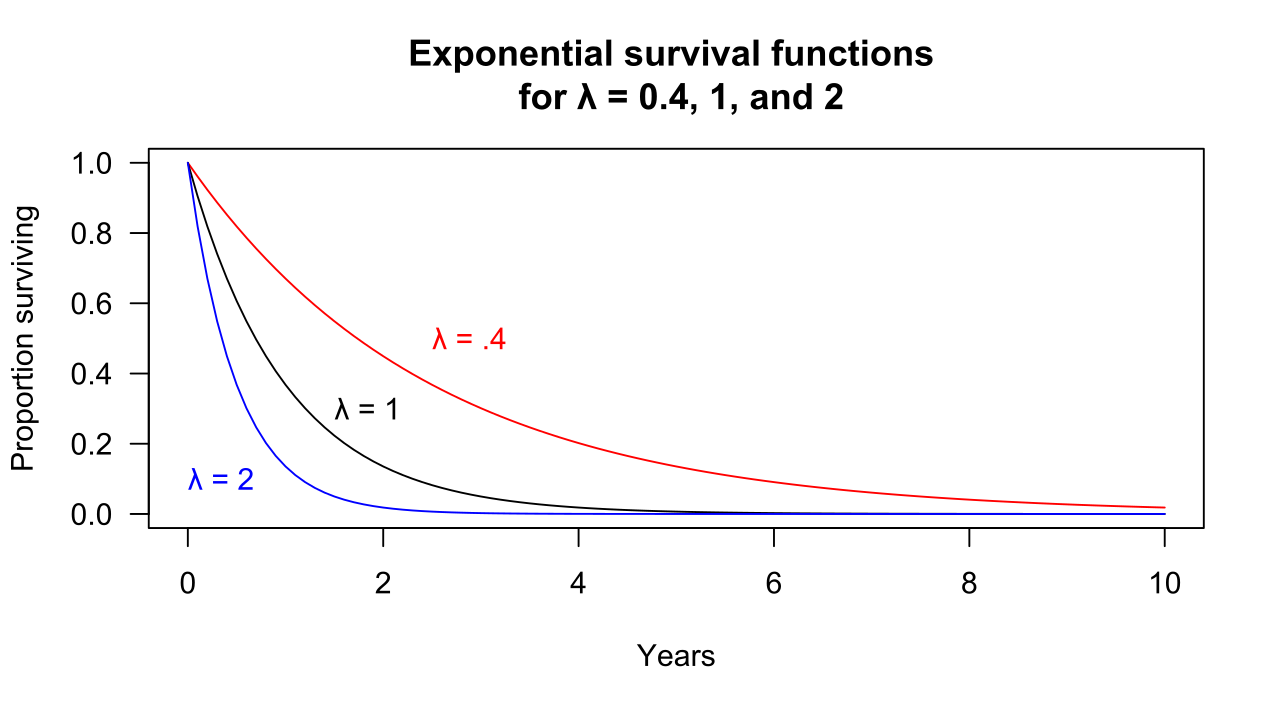
\includegraphics[width=0.78\textwidth]{Imagenes/modelo_exponencial_supervivencia.png}
    \caption[Ejemplo de funciones de supervivencia exponenciales]{Ejemplo de funciones de supervivencia exponenciales con distintos valores del parámetro $\lambda$. Fuente: Michaelg2015, Wikimedia Commons \cite{wikimedia_exponential_survival}.}
    \label{fig:modelo_exponencial_supervivencia}
\end{figure}

\subsection{Modelo de Weibull}
\paragraph*{}El modelo de Weibull es también un modelo paramétrico, pero ofrece mayor flexibilidad que el modelo exponencial. Su principal ventaja es que permite representar situaciones en las que el riesgo no permanece constante, sino que puede aumentar o disminuir a lo largo del tiempo \cite{davidsonpilon2019lifelines,jackson2016flexsurv}. Esa flexibilidad lo hace mucho más adecuado para capturar lo que realmente ocurre en las trayectorias académicas, donde el riesgo de abandono no es el mismo en el primer mes que en el tercer año.

\paragraph*{}Y es que la realidad es más complicada que una línea recta. Algunos estudiantes presentan mayor vulnerabilidad al principio, cuando todo es nuevo y la adaptación es más dura. Otros aguantan bien al inicio pero acumulan dificultades con el tiempo. Weibull puede capturar esos dos patrones, y eso lo convierte en una herramienta mucho más expresiva que el exponencial. Además, comparar los resultados de ambos modelos aporta información en sí misma: si Weibull ofrece un ajuste claramente mejor, es una señal de que el riesgo evoluciona con el tiempo y de que las estrategias de intervención deberían tenerlo en cuenta.

\begin{figure}[H]
    \centering
    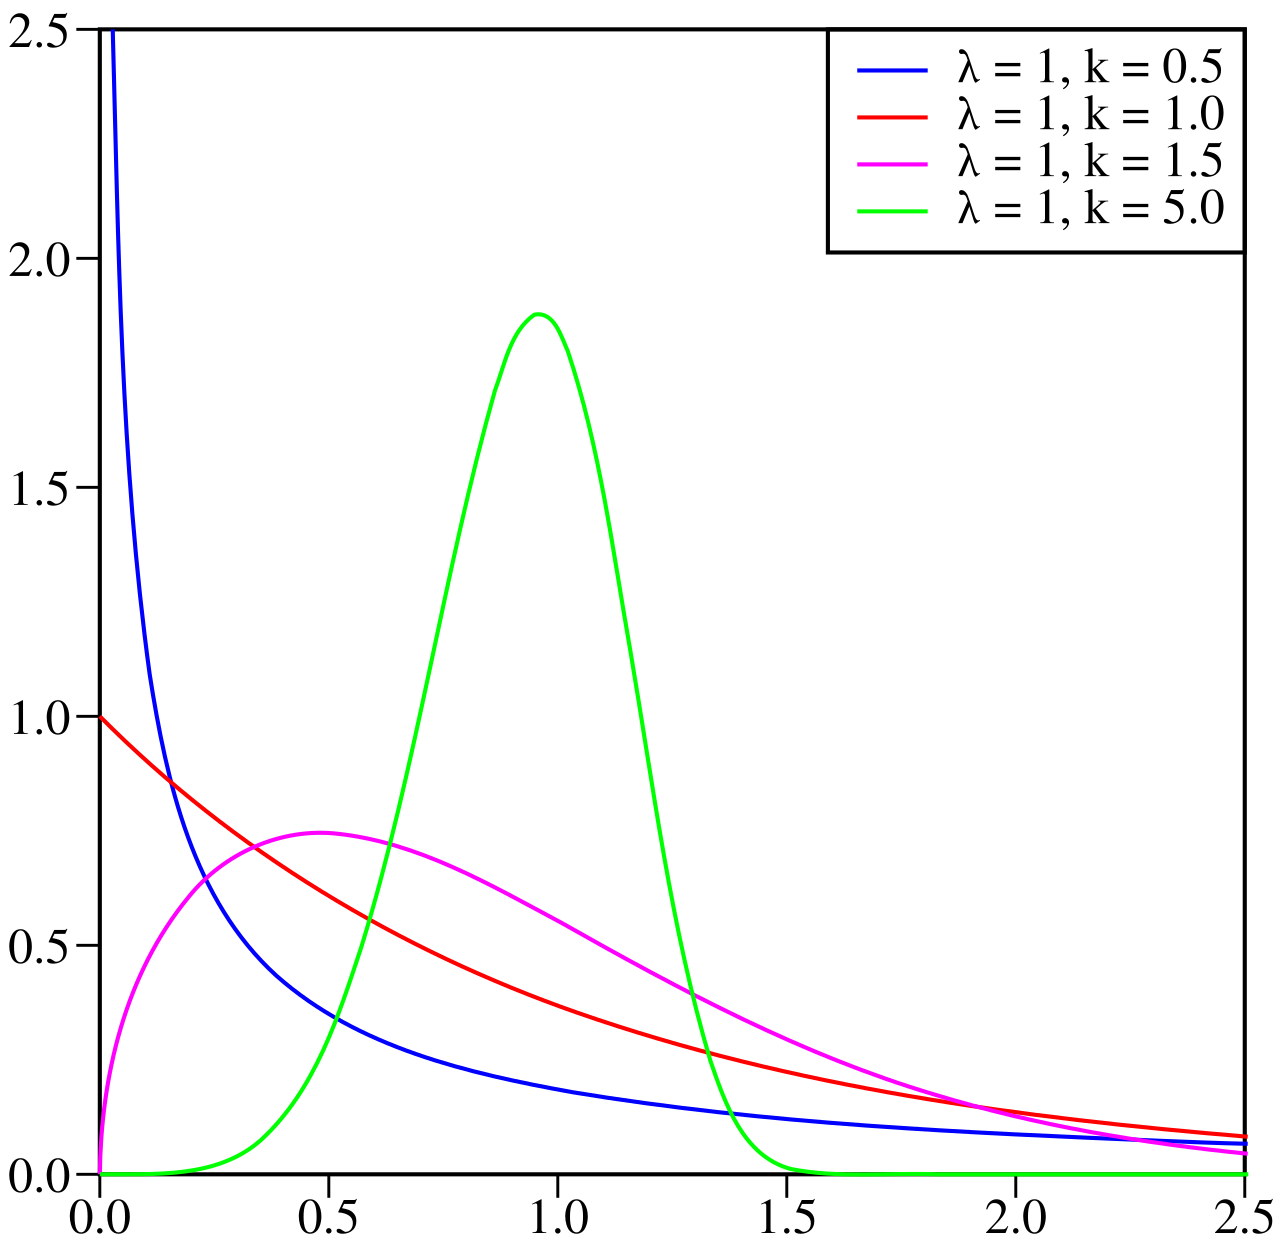
\includegraphics[width=0.40\textwidth]{Imagenes/modelo_weibull_pdf.png}
    \caption[Ejemplo de distribuciones de Weibull]{Ejemplo de distribuciones de Weibull con diferentes valores del parámetro de forma. Fuente: Calimo, Wikimedia Commons \cite{wikimedia_weibull_pdf}.}
    \label{fig:modelo_weibull_pdf}
\end{figure}

\subsection{Random Survival Forest}
\paragraph*{}Random Survival Forest es un salto cualitativo respecto a los modelos anteriores. Parte de la lógica de los bosques aleatorios, una técnica consolidada en aprendizaje automático, pero adaptada para trabajar con tiempos hasta evento y datos censurados \cite{ishwaran2008rsf}. Lo que lo distingue de todo lo anterior es que no exige asumir ninguna forma concreta para la función de supervivencia ni una relación lineal entre variables. Simplemente aprende de los datos.

\paragraph*{}Esa libertad tiene consecuencias prácticas importantes. En un fenómeno tan multifactorial como el abandono universitario, donde pueden intervenir al mismo tiempo el rendimiento, la situación personal, la carga académica y muchos otros factores, un modelo que capture relaciones complejas y no lineales puede detectar patrones que los métodos clásicos pasarían por alto. Además, Random Survival Forest ofrece algo especialmente útil para este proyecto: una medida de importancia de variables, que permite identificar qué factores pesan más en la predicción del abandono.

\paragraph*{}La contrapartida es que, a mayor complejidad, mayor necesidad de cautela. Los resultados de este modelo deben interpretarse con cuidado y, siempre que sea posible, contrastarse con los obtenidos por técnicas más transparentes. En este proyecto se implementa a través de \texttt{scikit-survival}, una librería especializada en análisis de tiempo hasta evento construida sobre el ecosistema de \texttt{scikit-learn} \cite{polsterl2020scikit}.
\begin{figure}[H]
    \centering
    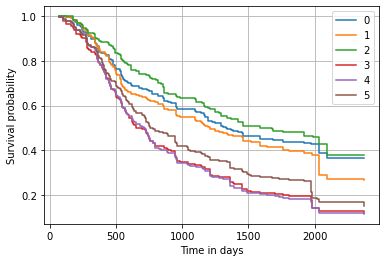
\includegraphics[width=0.72\textwidth]{Imagenes/random_survival_forest_predicciones.png}
    \caption[Ejemplo de curvas predichas mediante Random Survival Forest]{Ejemplo de curvas de supervivencia predichas mediante Random Survival Forest. Fuente: documentación oficial de scikit-survival \cite{scikit_survival_rsf}.}
    \label{fig:random_survival_forest_predicciones}
\end{figure}
